\section{Application: violent crime across U.S. communities}
\label{sec:realdata}

The analysis contains $n=1{,}993$ communities and $p=99$ candidate
predictors. Under the tuning selected in Section~\ref{sec:tuning},
$\alpha=n^{-0.3}\approx0.102$ and $h=n^{-0.1}/2\approx0.234$, so the
sample contains $n\alpha\approx204$ upper-tail observations in total and
about $2n\alpha h\approx95$ within a typical interior rank window
(no fewer than about $58$ near the trimmed boundary). The dimension
is therefore comparable to the number of observations available for
local tail estimation. Unrestricted or nonparametric joint tail
modelling with $99$ covariates is poorly supported by roughly $200$
upper-tail observations, and by fewer still within any local covariate
neighbourhood; a marginal screen can rank the $99$ candidates from
exactly this information.

\subsection{Data and protocol}

The Communities and Crime data set
\citep{redmond2002}, distributed by the UCI Machine Learning Repository
in its unnormalized version, links socio-economic census attributes,
law-enforcement survey attributes and FBI crime counts for $2{,}215$ U.S.
communities. The response is the violent-crime rate per $100{,}000$
inhabitants. We keep the communities with an observed positive response
($n=1{,}993$). Preprocessing of the $124$ documented predictive
attributes is response-blind: we retain numeric predictors with fewer
than $5\%$ missing values, which removes the $22$ law-enforcement
variables reported by only $343$ communities, and with at least $100$
distinct observed values, which removes $3$ low-cardinality variables,
keeping the application close to the continuous-marginal framework of
the theory. This leaves $p=99$
continuous predictors --- demographic composition, income and poverty,
education, employment, family structure, immigration, language, housing,
and population density. The at most one missing value per retained predictor is median-imputed,
and all three screens below work from the same imputed matrix.

The response is strongly right-skewed: median $374$, $99$th percentile
$2{,}943$, maximum $4{,}877$. The left panel of Figure~\ref{fig:crime}
shows the Hill curve of the response over $k\in[20,600]$ upper order
statistics; it is positive and moves slowly, between $0.283$ and
$0.374$ for $k\in[100,300]$, with value $0.328$ at the working level
$k=n\alpha=204$. The middle panel shows the Pareto QQ plot of the $600$
largest responses, approximately linear over the working range with
least-squares slope $0.27$. The gap between the QQ slope and the Hill
value at the same level ($0.33$) is mild evidence that regular
variation is only approximate over the working range. The response
exhibits a sufficiently heavy and stable upper tail to make a
tail-index analysis plausible; neither diagnostic establishes regular
variation beyond doubt, and no single threshold carries a structural
interpretation.

The screen uses $\alpha=n^{-0.3}$, $h=n^{-0.1}/2\approx0.234$,
$\varepsilon=0.05$. This tuning is the simulation-calibrated default of
Section~\ref{sec:tuning}; it is transferred to these data without any
claim that the crime-rate regime resembles the simulation designs, which
is why stability rather than a single fit carries the conclusions.
Stability is assessed three ways, none of which was used to choose the
tuning: the $3\times3$ grid
$a\in\{.25,.30,.35\}\times b\in\{.05,.10,.15\}$, which deliberately
includes the tail fraction $a=.25$ found fragile in simulation; $200$
seeded random half-samples refit with the primary rule; and $20$
randomized breakings of the few exact ties. The two competing screens of
Section~\ref{sec:comparison} are run on the same imputed matrix.

\subsection{Results}

Family structure dominates the ranking. The proportion of children in
two-parent households (\texttt{pctKids2Par}) ranks second in the primary
fit, within the top five in every tuning-grid fit, and in the top five of
$92\%$ of the $200$ half-samples --- the most stable variable in the
analysis. The related \texttt{pct2Par} and \texttt{pctKids4w2Par} and
the poverty rate \texttt{pctPoverty} behave similarly (top-five
frequencies $.64$, $.52$ and $.71$). These four variables are also
ranked highly by both competing screens (Yoshida--Umezu ranks $3$--$14$,
quantile SIS at $\tau=.95$ ranks $1$--$5$), so the three methods agree
that the body and the tail of the crime distribution share their main
covariates. The remaining primary top-ten variables
(\texttt{pctMaleNevMar}, \texttt{pct12to17w2Par},
\texttt{pctKidsBornNevrMarr}) sit in the same demographic cluster but
with lower half-sample stability (top-five frequencies $.21$--$.54$),
and \texttt{popDensity}, tenth in the primary fit, is unstable
(top-five frequency $.04$); we group all four with the candidates
rather than the findings.

The disagreements are the informative part. The share of workers using
public transportation (\texttt{pctUsePubTrans}) ranks first in the
primary fit and sixth in median over half-samples, yet ranks $57$th for
the Yoshida--Umezu screen and $53$rd for the quantile screen; the
farm-employment rate \texttt{pctWfarm} shows the same pattern (rank $5$
against $60$ and $59$). These predictors receive relatively strong
tail-index screening scores while ranking much lower under the
$0.95$-quantile screen: their low scores are consistent with marginal
variation in upper-tail heaviness across their values, of a kind that a
fixed-quantile screen is not designed to detect.
Section~\ref{sec:comparison} produces the same dissociation under
controlled conditions, where the target is known. Both variables are, however, clearly less stable
than the family-structure block: their top-five half-sample frequencies
are $.44$ and $.35$, their 10--90\% half-sample rank intervals are
$[1,14]$ and $[2,19]$, and their worst ranks over the $3\times3$ tuning
grid are $20$ and $18$, driven by the $a=.25$ fits. We report them as candidate tail-specific predictors for the
second-stage analysis to examine.

Ranks are insensitive to tie breaking (maximal displacement over $20$
randomized fits: one position for the leaders). We do not interpret any
ranking causally: the screen identifies covariates along which the
conditional tail index varies marginally, and confounding among the $99$
predictors is certain.

\begin{figure}[t]
\centering
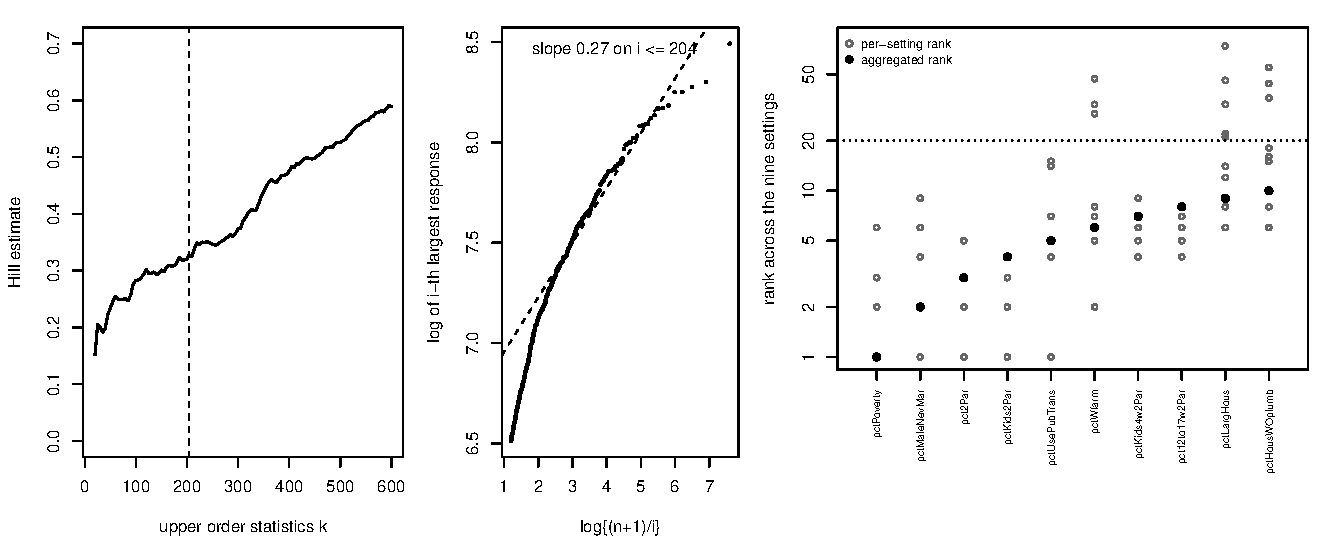
\includegraphics[width=.98\linewidth]{figures/crime_application.pdf}
\caption{Communities and Crime application ($n=1{,}993$, $p=99$,
$\alpha=n^{-0.3}$, $h=n^{-0.1}/2$). Left: Hill estimates for the
violent-crime rate; the dashed line marks the working level
$k=n\alpha=204$. Middle: Pareto QQ plot of the $600$ largest responses;
the dashed line is fitted over the working range $i\le204$. Right:
distribution of the ranks of the ten leading predictors over $200$
seeded half-samples; the dotted line is the default retained size
$d=20$.}
\label{fig:crime}
\end{figure}
